% Chapter 6: Spectral Analysis
% ASSUMES: Chapter 5 defines H(s), H_z, H_0, |psi_0>, A_p, A_1, A_2,
%   s^*, delta_s, g_min, hat{g}, the three regions, symmetric states |k>,
%   eigenvalue equation (Lemma 5.1), validity of approximation (Lemma 5.2),
%   gap in window (Lemma 5.3), gap-left-preview (Lemma 5.4),
%   gap-right-preview (Lemma 5.5), Delta = E_1 - E_0.

Chapter 5 established the crossing window $\mathcal{I}_{s^*}$ where the spectral gap satisfies $g(s) = \Theta(g_{\min})$, and stated two bounds for the regions outside: a linear lower bound to the left (\autoref{lem:gap-left-preview}) and a linear lower bound to the right (\autoref{lem:gap-right-preview}). The complete gap profile determines the runtime of the adiabatic algorithm through the integral $\int_0^1 g(s)^{-2}\, ds$: a piecewise linear lower bound on $g(s)$ makes this integral tractable, splitting it into three closed-form pieces whose relative contributions identify the bottleneck. This chapter proves both lemmas.

The two proofs use different techniques, reflecting different spectral structures on each side of the crossing. To the left of $s^*$, the ground energy $\lambda_0(s)$ sits below $sE_0$ while the first excited energy $\lambda_1(s)$ sits above it. The variational principle bounds how far below $sE_0$ the ground energy can be, yielding a linear gap bound. To the right of $s^*$, the eigenvalues of $sH_z$ crowd the interval $[sE_0, sE_1]$, and the variational approach no longer applies. Instead, a resolvent identity combined with the Sherman-Morrison formula for rank-one perturbations tracks the gap through this congested region. The resulting piecewise linear profile --- steep on the left, shallower on the right, flat in the window --- feeds directly into the runtime calculation of Chapter 7.

\section{Gap to the Left of the Crossing}
\label{sec:gap-left}

The eigenvalue equation (\autoref{lem:eigenvalue-equation}) places the ground state energy at $\lambda_0(s) < sE_0$ and the first excited energy at $\lambda_1(s) \in (sE_0, sE_1)$. The gap $g(s) = \lambda_1(s) - \lambda_0(s)$ is therefore positive, but these bounds alone give only the trivial estimate $g(s) < s\Delta$. For the runtime integral, we need a tight lower bound that captures the linear growth of the gap as $s$ decreases away from $s^*$.

The strategy is to tighten the upper bound on $\lambda_0(s)$. Two approaches give the same result. The first uses the variational principle: for any normalized state $\ket{\phi}$, the ground energy satisfies $\lambda_0(s) \leq \bra{\phi}H(s)\ket{\phi}$, so a well-chosen ansatz produces a quantitative upper bound. The second uses concavity: since $\lambda_0(s) = \min_{\ket{\psi}} \bra{\psi} H(s) \ket{\psi}$ is the pointwise minimum of affine functions in $s$, it is concave, and any tangent line lies above it. The variational approach is more direct --- it produces the bound in a single calculation --- so we present it here.

\begin{lemma}[Gap to the left of the crossing]
\label{lem:gap-left}
For any $s \in \mathcal{I}_{s^\leftarrow} = [0, \, s^* - \delta_s)$, the spectral gap of $H(s)$ satisfies
\begin{equation}
\label{eq:gap-left}
g(s) \geq \frac{A_1(A_1 + 1)}{A_2}\left(s^* - s\right).
\end{equation}
\end{lemma}

\begin{proof}
We upper-bound $\lambda_0(s)$ via the variational principle and lower-bound $\lambda_1(s)$ from the eigenvalue equation.

The ansatz must live in the span of $\{\ket{k} : k \geq 1\}$, orthogonal to the ground-state component $\ket{0}$, and should concentrate amplitude on levels close to $E_0$ where the energy expectation is lowest. The natural weighting is the inverse energy gap: levels near $E_0$ receive more amplitude. Requiring unit norm fixes the overall scale, giving
\begin{equation}
\label{eq:ansatz-left}
\ket{\phi} = \frac{1}{\sqrt{A_2 N}} \sum_{k=1}^{M-1} \frac{\sqrt{d_k}}{E_k - E_0}\,\ket{k}.
\end{equation}
This weighting arises naturally in first-order perturbation theory: the correction to the ground state $\ket{E_0}$ of $sH_z$ due to the perturbation $-(1-s)\ket{\psi_0}\bra{\psi_0}$ has coefficients proportional to $\braket{E_k}{\psi_0}/(E_k - E_0) = \sqrt{d_k/N}/(E_k - E_0)$, which is exactly the form above up to normalization. Normalization is immediate:
\begin{equation}
\braket{\phi}{\phi} = \frac{1}{A_2 N} \sum_{k=1}^{M-1} \frac{d_k}{(E_k - E_0)^2} = \frac{A_2}{A_2} = 1.
\end{equation}

To compute $\bra{\phi}H(s)\ket{\phi}$, decompose $H(s) = -(1-s)\ket{\psi_0}\bra{\psi_0} + s(H_z - E_0) + sE_0$. Each term contributes separately.

The projector term gives
\begin{equation}
-(1-s)\left|\braket{\psi_0}{\phi}\right|^2 = -(1-s)\left(\frac{1}{\sqrt{A_2 N}} \sum_{k=1}^{M-1} \frac{d_k}{(E_k - E_0)\sqrt{N}}\right)^{\!2} = -(1-s)\frac{A_1^2}{A_2},
\end{equation}
where $\braket{\psi_0}{\phi} = A_1/\sqrt{A_2}$ follows from $\braket{\psi_0}{k} = \sqrt{d_k/N}$ and the definition of $A_1$.

The shifted diagonal term gives
\begin{equation}
s\bra{\phi}(H_z - E_0)\ket{\phi} = \frac{s}{A_2 N} \sum_{k=1}^{M-1} \frac{d_k}{(E_k - E_0)^2} \cdot (E_k - E_0) = \frac{s}{A_2 N}\sum_{k=1}^{M-1} \frac{d_k}{E_k - E_0} = \frac{s\, A_1}{A_2}.
\end{equation}

The constant term contributes $sE_0 \braket{\phi}{\phi} = sE_0$. Combining:
\begin{equation}
\label{eq:variational-bound}
\lambda_0(s) \leq \bra{\phi}H(s)\ket{\phi} = sE_0 - (1-s)\frac{A_1^2}{A_2} + s\frac{A_1}{A_2} = sE_0 + \frac{A_1}{A_2}\left(s(1 + A_1) - A_1\right).
\end{equation}
Since $s^*(1 + A_1) = A_1$, we have $s(1+A_1) - A_1 = (1+A_1)(s - s^*) = (s-s^*)/(1-s^*)$, so
\begin{equation}
\label{eq:lambda0-upper}
\lambda_0(s) \leq sE_0 + \frac{A_1}{A_2}\cdot\frac{s - s^*}{1 - s^*}.
\end{equation}
For $s < s^*$, the second term is negative, confirming $\lambda_0(s) < sE_0$.

For the first excited state, the eigenvalue equation (\autoref{lem:eigenvalue-equation}) confines $\lambda_1(s)$ to the interval $(sE_0, sE_1)$, so
\begin{equation}
\lambda_1(s) \geq sE_0.
\end{equation}

The gap is therefore
\begin{equation}
g(s) = \lambda_1(s) - \lambda_0(s) \geq sE_0 - sE_0 - \frac{A_1}{A_2}\cdot\frac{s - s^*}{1 - s^*} = \frac{A_1}{A_2}\cdot\frac{s^* - s}{1 - s^*}.
\end{equation}
Since $1/(1-s^*) = A_1 + 1$, we obtain $g(s) \geq A_1(A_1 + 1)(s^* - s)/A_2$.
\end{proof}

At the left boundary of the crossing window, $s = s^* - \delta_s$, the bound gives
\begin{equation}
g(s^* - \delta_s) \geq \frac{A_1(A_1+1)}{A_2}\cdot\delta_s = \hat{g},
\end{equation}
using $A_1(A_1+1)\delta_s/A_2 = \hat{g}$ from Eq.~\eqref{eq:gmin-deltas-relation}. Since $g_{\min} = (1 \pm O(\eta))\hat{g}$ from Eq.~\eqref{eq:gmin-formula}, the gap at the window boundary is $\Theta(g_{\min})$, confirming that the piecewise bounds are consistent across regions and that the minimum gap lies within $\mathcal{I}_{s^*}$.

An alternative derivation uses concavity. Since $\lambda_0(s) = \min_{\ket{\psi}} \bra{\psi} H(s) \ket{\psi}$ is the pointwise minimum of affine functions in $s$, it is concave. The Hellmann-Feynman theorem gives the second derivative explicitly:
$$\ddot{\lambda}_0(s) = -2\sum_{j \geq 1} \frac{|\bra{\phi_j(s)}\dot{H}\ket{\phi_0(s)}|^2}{\lambda_j(s) - \lambda_0(s)} \leq 0,$$
where $\dot{H} = H_z + \ket{\psi_0}\bra{\psi_0}$ and $\ket{\phi_j(s)}$ are the instantaneous eigenstates. Concavity implies any tangent lies above the function: the tangent to $\lambda_0$ at $s^*$ gives $\lambda_0(s) \leq \lambda_0(s^*) + \lambda_0'(s^*)(s - s^*)$, an upper bound of the same form as~\eqref{eq:lambda0-upper}, though the variational approach gives slightly sharper constants.

For the running example ($M = 2$, $d_0 = 1$, $d_1 = N-1$, $E_0 = 0$, $E_1 = 1$), the ansatz reduces to $\ket{\phi} = \ket{1}$, and the bound becomes
\begin{equation}
g(s) \geq \frac{(N-1)/N \cdot (2N-1)/N}{(N-1)/N}\left(\frac{1}{2} - s\right) = \frac{2N - 1}{N}\left(\frac{1}{2} - s\right) \approx 2\left(\frac{1}{2} - s\right).
\end{equation}
The exact gap $g(s) = \sqrt{(2s-1)^2 + 4s(1-s)/N}$ at $s = 1/4$ equals $\sqrt{1/4 + 3/(4N)} \approx 1/2$, while the bound gives $(2N-1)/(4N) \approx 1/2$. The bound is tight near $s^*$ and only becomes loose as $s$ approaches $0$, where the true gap approaches $1$ while the bound continues growing. Since the runtime integral is dominated by the crossing window, this looseness far from $s^*$ has negligible effect.

\section{Gap to the Right of the Crossing}
\label{sec:gap-right}

Bounding the spectral gap to the right of $s^*$ is the main technical challenge of this chapter. The variational principle that worked on the left does not extend: it provides upper bounds on $\lambda_0(s)$, but what we need on the right is a lower bound on $\lambda_1(s) - \lambda_0(s)$ that captures the linear reopening of the gap. The variational principle bounds ground energies from above, not excited energies from below.

The obstacle is structural. On the left, the first excited eigenvalue $\lambda_1(s)$ is bounded below by $sE_0$ from the eigenvalue equation, giving a clean reference point. On the right, $\lambda_1(s)$ lies between $sE_0$ and $sE_1$, but so do eigenvalues from the higher levels of $sH_z$, which undergo their own avoided crossings with the first excited state. Tracking $\lambda_1(s)$ through this congested region requires a tool that bounds the distance from a given point to the spectrum without identifying individual eigenvalues. The eigenvalue equation (\autoref{lem:eigenvalue-equation}) characterizes the full spectrum implicitly --- each eigenvalue satisfies a transcendental equation --- but it does not yield a closed-form bound on any individual eigenvalue that captures the gap's linear dependence on $s - s^*$.

The resolvent provides exactly this. For a self-adjoint operator $A$ with spectrum $\sigma(A)$ and any $\lambda \notin \sigma(A)$, the resolvent
\begin{equation}
\label{eq:resolvent-def}
R_A(\lambda) = (\lambda I - A)^{-1}
\end{equation}
is a bounded operator whose norm equals the inverse distance from $\lambda$ to the spectrum:
\begin{equation}
\label{eq:resolvent-norm}
\lVert R_A(\lambda) \rVert = \frac{1}{\mathrm{dist}(\lambda,\, \sigma(A))}.
\end{equation}
This follows from the spectral theorem: in the eigenbasis of $A$ with eigenvalues $\{\lambda_j\}$, the resolvent is diagonal with entries $1/(\lambda - \lambda_j)$, and its operator norm is the maximum absolute value $\max_j |1/(\lambda - \lambda_j)| = 1/\min_j|\lambda - \lambda_j|$. If a point $\gamma$ lies between two consecutive eigenvalues $\lambda_0$ and $\lambda_1$, then $\mathrm{dist}(\gamma, \sigma(A)) = \min(\gamma - \lambda_0, \lambda_1 - \gamma) \leq g/2$, since the minimum of two non-negative numbers summing to $g$ is at most $g/2$. Therefore $\lVert R_A(\gamma) \rVert = 1/\mathrm{dist}(\gamma, \sigma(A)) \geq 2/g$, and the useful contrapositive is
\begin{equation}
\label{eq:gap-resolvent}
g(s) \geq \frac{2}{\lVert R_{H(s)}(\gamma) \rVert}.
\end{equation}
Bounding the gap from below reduces to bounding the resolvent norm from above. This resolvent approach to rank-one perturbations has precedent in the spatial search literature. Childs and Goldstone~\cite{childs2004spatial} showed that a continuous-time quantum walk on the complete graph finds a marked vertex in $O(\sqrt{N})$ time by analyzing the resolvent of the graph Laplacian perturbed by a rank-one oracle projector --- the same algebraic structure as our adiabatic Hamiltonian $H(s) = sH_z - (1-s)\ket{\psi_0}\bra{\psi_0}$, with the Laplacian replaced by the diagonal problem Hamiltonian. Chakraborty, Novo, and Roland~\cite{chakraborty2020optimality} extended this to general graphs, proving optimality of spatial search for almost all graphs using the Sherman-Morrison identity to bound the resolvent of rank-one perturbations. Their technique transfers directly to the adiabatic setting: the algebraic steps are identical, with the spectral parameters $A_1$, $A_2$ replacing the graph-theoretic quantities.

The parallel merits a closer look, because the reader who understands it will recognize the resolvent technique as a general tool rather than a problem-specific trick. Spatial search via continuous-time quantum walks solves the following problem: given a graph $G$ on $N$ vertices with a subset $S$ of marked vertices, find a marked vertex by evolving the initial state $\ket{s} = (1/\sqrt{N})\sum_v \ket{v}$ under the Hamiltonian $H_{\text{search}} = -\gamma L - \sum_{v \in S}\ket{v}\bra{v}$, where $L$ is the graph Laplacian and $\gamma > 0$ is a tunable parameter \cite{childs2004spatial}. The oracle term $-\sum_{v \in S}\ket{v}\bra{v}$ is a rank-one projector when $|S| = 1$ (or more generally a low-rank perturbation), and the Laplacian $L$ plays the role of the diagonal Hamiltonian $sH_z$: its eigenvalues are the graph's spectrum, and the spectral gap of $L$ determines the time scale of the walk. The mapping is: $L \leftrightarrow sH_z$, the oracle projector $\leftrightarrow (1-s)\ket{\psi_0}\bra{\psi_0}$, the algebraic connectivity of $G$ $\leftrightarrow$ the spectral gap $\Delta$ of $H_z$, and the effective resistance at the marked vertex $\leftrightarrow$ the spectral parameter $A_2$. The resolvent bound proceeds identically in both settings: place a line $\gamma(s)$ between the two lowest eigenvalues, apply the Sherman-Morrison formula to decompose the resolvent of the rank-one perturbation into the known resolvent of the diagonal operator plus a correction, and bound the correction using the spectral parameters. The reason this works is structural: rank-one perturbations of diagonal operators admit Sherman-Morrison inversion regardless of the dimension or the specific eigenvalue distribution, reducing the spectral gap problem to bounding a single rational function of the parameters.

The connection also explains why the same constants ($k = 1/4$, $f(s^*) = 4$) appear in both analyses. These values are artifacts of the line-placement optimization --- balancing the denominator's positivity against the numerator's growth in the function $f(s)$ --- and depend only on the rank-one structure, not on whether the underlying operator is a graph Laplacian or a problem Hamiltonian. Any future application of this technique to a new rank-one perturbation will face the same optimization, with the same constants serving as a starting point.

Since $H(s) = sH_z - (1-s)\ket{\psi_0}\bra{\psi_0}$ is a rank-one perturbation of $sH_z$, we can invert its resolvent explicitly. The Sherman-Morrison identity \cite{sherman_morrison} states that for an invertible operator $A$ and vectors $\ket{u}, \bra{v}$,
\begin{equation}
\label{eq:sherman-morrison}
(A + \ket{u}\bra{v})^{-1} = A^{-1} - \frac{A^{-1}\ket{u}\bra{v}A^{-1}}{1 + \bra{v}A^{-1}\ket{u}},
\end{equation}
provided $1 + \bra{v}A^{-1}\ket{u} \neq 0$. Applying this to the resolvent of $H(s)$ decomposes it into the resolvent of $sH_z$ (whose spectrum is known explicitly) and a correction from the rank-one term $-(1-s)\ket{\psi_0}\bra{\psi_0}$. The triangle inequality then yields an upper bound on $\lVert R_{H(s)}(\gamma)\rVert$.

The strategy is: choose a line $\gamma(s)$ that lies between $\lambda_0(s)$ and $\lambda_1(s)$ for all $s \geq s^*$, apply the Sherman-Morrison decomposition, bound each piece using the spectral parameters $A_1$ and $A_2$, and show that the resulting bound on $\lVert R_{H(s)}(\gamma)\rVert$ yields a linear lower bound on $g(s)$.

The simplest choice for $\gamma(s)$ is a line starting at $sE_0$ when $s = s^*$ and ending between $E_0$ and $E_1$ at $s = 1$: take $\beta(s) = a(s - s^*)/(1 - s^*)$ with $a < \Delta$ and set $\gamma(s) = sE_0 + \beta(s)$. With $a = \Delta/6$, the function $f(s)$ controlling the resolvent bound can be shown to satisfy $f(s) \leq 1$ for all $s \geq s^*$, giving $g(s) \geq \beta(s) = (\Delta/6)(s - s^*)/(1 - s^*)$. This bound has a problem: at the window boundary $s = s^* + \delta_s$, it gives $g(s^*+\delta_s) \geq (\Delta/6) \cdot \delta_s/(1-s^*) = (\Delta A_2)/(6A_1) \cdot g_{\min}$. Since $\Delta A_2 \leq A_1$, this is at most $g_{\min}/6$, and for Hamiltonians with $\Delta A_2 \ll A_1$, it can be polynomially smaller than $g_{\min}$. At $s = s^*$ itself, the bound gives $g(s^*) \geq 0$, missing the true gap entirely.

The failure has a geometric explanation. At $s^*$, the ground energy $\lambda_0(s^*)$ is not at $s^*E_0$ but rather $g_{\min}/2$ below it. The line $\gamma(s)$ passes through $s^*E_0$ at $s = s^*$, so it sits between the two eigenvalues but with zero margin below. The resolvent norm at a point equidistant from two eigenvalues has norm $2/g$, but at a point touching one eigenvalue, the norm diverges. The line must start with $O(g_{\min})$ separation from both eigenvalues at $s^*$.

The fix is to shift the line's origin from $s^*$ to a point $s_0 < s^*$ so that $\beta(s^*) = k\, g_{\min}$ for a constant $k < 1$. With $\beta(s) = a(s - s_0)/(1 - s_0)$, the constraint $\beta(s^*) = k\,g_{\min}$ determines
\begin{equation}
\label{eq:s0-definition}
s_0 = s^* - \frac{k\, g_{\min}(1 - s^*)}{a - k\, g_{\min}}.
\end{equation}
The line now passes through $\gamma(s^*) = s^*E_0 + k\,g_{\min}$, which lies between $\lambda_0(s^*)$ and $\lambda_1(s^*)$ when $k$ is chosen appropriately. The price is that $s_0 < s^*$ introduces additional terms in the monotonicity analysis for $f(s)$, requiring a careful choice of $a$.

\begin{lemma}[Gap to the right of the crossing]
\label{lem:gap-right}
Assume $A_1 \geq 1/2$. Let $k = 1/4$, $a = 4k^2\Delta/3 = \Delta/12$, and $s_0$ as in Eq.~\eqref{eq:s0-definition}. Then for all $s \geq s^*$, the spectral gap of $H(s)$ satisfies
\begin{equation}
\label{eq:gap-right}
g(s) \geq \frac{\Delta}{30}\cdot\frac{s - s_0}{1 - s_0}.
\end{equation}
\end{lemma}

\begin{proof}
Set $\gamma(s) = sE_0 + \beta(s)$ with $\beta(s) = a(s - s_0)/(1-s_0)$. We bound $\lVert R_{H(s)}(\gamma)\rVert$ from above using the Sherman-Morrison formula.

Since $H(s) = sH_z - (1-s)\ket{\psi_0}\bra{\psi_0}$, the resolvent of $H(s)$ at $\gamma$ satisfies, via Eq.~\eqref{eq:sherman-morrison} and the triangle inequality,
\begin{equation}
\label{eq:resolvent-SM}
\lVert R_{H(s)}(\gamma)\rVert \leq \lVert R_{sH_z}(\gamma)\rVert + (1-s)\frac{\lVert R_{sH_z}(\gamma)\ket{\psi_0}\bra{\psi_0}R_{sH_z}(\gamma)\rVert}{1 + (1-s)\bra{\psi_0}R_{sH_z}(\gamma)\ket{\psi_0}}.
\end{equation}

The unperturbed resolvent $R_{sH_z}(\gamma)$ is diagonal in the $\ket{k}$ basis with entries $1/(\gamma - sE_k) = 1/(\beta - s(E_k - E_0))$ for $k \geq 1$ and $1/\beta$ for $k = 0$. The nearest eigenvalue of $sH_z$ to $\gamma$ is $sE_0$, at distance $\beta$, so $\lVert R_{sH_z}(\gamma)\rVert = 1/\beta$.

We bound the numerator and denominator of the second term separately. Both require that $\beta(s) \leq s(E_k - E_0)/2$ for all $k \geq 1$, which ensures the Taylor expansion in powers of $\beta/(s(E_k - E_0))$ converges rapidly. Since $\beta(s) \leq a = \Delta/12$ and $s(E_k - E_0) \geq s^*\Delta \geq \Delta/3$ (using $s^* = A_1/(A_1+1) \geq 1/3$, which holds when $A_1 \geq 1/2$), we have $\beta \leq \Delta/12 < \Delta/6 \leq s(E_k - E_0)/2$. The condition $A_1 \geq 1/2$ requires that the spectral gaps $E_k - E_0$ are not too large relative to $d_0$; when $A_1 < 1/2$, the crossing occurs at $s^* < 1/3$ and the ground-state degeneracy $d_0$ is large enough that random sampling finds a solution with constant probability, making the adiabatic approach unnecessary.

\textbf{Numerator bound.} The squared norm of $R_{sH_z}(\gamma)\ket{\psi_0}$ expands as
\begin{equation}
\lVert R_{sH_z}(\gamma)\ket{\psi_0}\rVert^2 = \frac{d_0}{N\beta^2} + \frac{1}{N}\sum_{k=1}^{M-1}\frac{d_k}{\left(s(E_k - E_0) - \beta\right)^2}.
\end{equation}
Using $s(E_k - E_0) - \beta \geq s(E_k - E_0)/2$, each term in the sum is at most $4d_k/(Ns^2(E_k - E_0)^2)$, giving
\begin{equation}
\label{eq:numerator-bound}
\lVert R_{sH_z}(\gamma)\ket{\psi_0}\bra{\psi_0} R_{sH_z}(\gamma)\rVert \leq \lVert R_{sH_z}(\gamma)\ket{\psi_0}\rVert^2 \leq \frac{d_0}{N\beta^2} + \frac{4A_2}{s^2}.
\end{equation}

\textbf{Denominator bound.} Expanding the expectation value:
\begin{align}
1 + (1-s)\bra{\psi_0}R_{sH_z}(\gamma)\ket{\psi_0} &= 1 + \frac{(1-s)d_0}{N\beta} - \frac{1-s}{N}\sum_{k=1}^{M-1}\frac{d_k}{s(E_k - E_0) - \beta} \nonumber \\
&= 1 + \frac{(1-s)d_0}{N\beta} - \frac{1-s}{s}\sum_{k=1}^{M-1}\frac{d_k}{N(E_k - E_0)}\sum_{\ell=0}^{\infty}\left(\frac{\beta}{s(E_k - E_0)}\right)^{\!\ell}.
\end{align}
Using $\beta/(s(E_k - E_0)) \leq 1/2$ to bound the geometric series by $1 + 2\beta/(s(E_k - E_0))$:
\begin{equation}
\label{eq:denominator-bound}
1 + (1-s)\bra{\psi_0}R_{sH_z}(\gamma)\ket{\psi_0} \geq 1 + \frac{(1-s)d_0}{N\beta} - (1-s)\left(\frac{A_1}{s} + \frac{2A_2\beta}{s^2}\right).
\end{equation}

\textbf{Collecting terms.} Substituting the bounds~\eqref{eq:numerator-bound} and~\eqref{eq:denominator-bound} into~\eqref{eq:resolvent-SM} and factoring:
\begin{equation}
\label{eq:resolvent-f}
\lVert R_{H(s)}(\gamma)\rVert \leq \frac{1}{\beta}\left(1 + f(s)\right),
\end{equation}
and
\begin{equation}
\label{eq:f-definition}
f(s) = \frac{\frac{d_0}{N}\, s^2(1-s) + 4A_2\beta^2(1-s)}{\frac{d_0}{N}\, s^2(1-s) + \beta\, s\,\dfrac{s - s^*}{1 - s^*} - 2A_2\beta^2(1-s)}.
\end{equation}
To obtain this form, multiply numerator and denominator of the second term in~\eqref{eq:resolvent-SM} by $\beta$, then multiply by $s^2(1-s)$ to clear fractions. The key step is rewriting the denominator's constant-plus-linear terms. Using $A_1 = s^*/(1-s^*)$:
\begin{equation}
1 - \frac{(1-s)A_1}{s} + \frac{(1-s)d_0}{N\beta} = \frac{s - s^*}{s(1-s^*)} + \frac{(1-s)d_0}{N\beta},
\end{equation}
since $1 - A_1(1-s)/s = (s - A_1(1-s))/s = (s - s^*(1-s)/(1-s^*))/s = (s(1-s^*) - s^*(1-s))/(s(1-s^*)) = (s-s^*)/(s(1-s^*))$. Multiplying through by $\beta s^2(1-s)$ and collecting the Taylor-bounded terms into the $A_2\beta^2$ contributions gives Eq.~\eqref{eq:f-definition}. The fraction $d_0/N$ measures the density of ground states in the computational basis.

The numerator of $f(s)$ measures the rank-one perturbation's effect on the resolvent: the $d_0/N$ term comes from the $\ket{0}$ component of $\ket{\psi_0}$ (the ground-state overlap), while the $A_2$ term comes from the excited components. The denominator captures the spectral rigidity: the term $\beta\,s(s-s^*)/(1-s^*)$ grows as $\gamma$ moves away from the crossing, stabilizing the resolvent against the perturbation. Near $s^*$, the denominator is small (the gap is small), so $f(s^*)$ is $O(1)$. As $s$ increases, the denominator grows and $f(s) \to 0$.

From~\eqref{eq:resolvent-f} and~\eqref{eq:gap-resolvent}, the spectral gap satisfies
\begin{equation}
\label{eq:gap-via-f}
g(s) \geq \frac{2\beta(s)}{1 + f(s)} \geq \frac{2\beta(s)}{1 + \max_{s \geq s^*} f(s)}.
\end{equation}
If $f$ is monotonically decreasing on $[s^*, 1]$, then $\max_{s \geq s^*} f(s) = f(s^*)$, and the bound becomes $g(s) \geq 2\beta(s)/(1 + f(s^*))$, which is linear in $s - s_0$.

\textbf{Monotonicity of $f$.} We show $f'(s) < 0$ for $s \in [s^*, 1]$. Writing $f = u/v$, the sign of $f'$ is determined by $u'v - uv'$. After expanding and cancelling common terms, the expression reduces to three contributions: two are manifestly negative, while a third --- positive and proportional to $(d_0/N)\,s_0$ --- arises from having shifted the line's origin below $s^*$. The proof amounts to showing the negative terms dominate. Write $f = u/v$ with
\begin{align}
\label{eq:uv-def}
u &= \frac{d_0}{N}\,s^2(1-s) + 4A_2\beta^2(1-s), \\
v &= \frac{d_0}{N}\,s^2(1-s) + \beta\,s\,\frac{s - s^*}{1-s^*} - 2A_2\beta^2(1-s). \nonumber
\end{align}
Then $f' = (u'v - uv')/v^2$, so the sign of $f'$ is determined by $u'v - uv'$.

Computing $u'$ and $v'$ using $\beta' = a/(1-s_0)$:
\begin{align}
u' &= \frac{4aA_2\beta}{1-s_0}(2 + s_0 - 3s) + \frac{d_0}{N}\, s(2 - 3s), \label{eq:u-prime} \\
v' &= \frac{a(3s^2 - 2s(s^* + s_0) + s^*s_0)}{(1-s_0)(1-s^*)} - \frac{2aA_2\beta}{1-s_0}(2 + s_0 - 3s) + \frac{d_0}{N}\,s(2-3s). \nonumber
\end{align}

Expanding $u'v$ and $uv'$ and taking the difference, two terms cancel exactly: the $(d_0/N)^2 s^3(2-3s)(1-s)$ term and the $8a A_2^2\beta^3(1-s)(2+s_0-3s)/(1-s_0)$ term. The remaining expression has three terms \cite{braida2024unstructured}:
\begin{align}
\label{eq:upv-uvp}
u'v - uv' =\;& -\frac{4aA_2\beta^2}{(1-s_0)(1-s^*)}\Big(s^2(1 + s_0 - s^*) - 2s\,s_0 + s^*s_0\Big) \\
&+ \frac{12aA_2\frac{d_0}{N}\,\beta}{1-s_0}\,s(1-s)^2\,s_0 \nonumber \\
&- \frac{\frac{d_0}{N}\,s^2 a}{(1-s_0)(1-s^*)}\Big({-}s^2(s^* + s_0 - 1) + 2s\,s_0 s^* - s^*s_0\Big). \nonumber
\end{align}
The first and third terms are negative; the second is positive (it is the only term involving $(d_0/N)\,s_0$, which arises from the shift of $s_0$ below $s^*$). We must show the first negative term dominates the positive one.

Factor out $-4aA_2\beta/(1-s_0)$ from the sum of the first two terms:
\begin{equation}
\label{eq:domination-argument}
-\frac{4aA_2\beta}{1-s_0}\left(\frac{\beta}{1-s^*}\Big(s^2(1+s_0-s^*) - 2s\,s_0 + s^*s_0\Big) - \frac{3d_0}{N}\,s_0\,s(1-s)^2\right).
\end{equation}
The quadratic $s^2(1+s_0-s^*) - 2s\,s_0 + s^*s_0$ is a convex function of $s$ (the leading coefficient $1+s_0-s^* > 0$ since $s_0 < s^*$), minimized at some $s_m < s^*$, and positive for $s \geq s^*$: at $s = s^*$, it evaluates to $s^*(1-s^*)(s^*-s_0) > 0$. The cubic $s(1-s)^2$ is maximized at $s = 1/3 \leq s^*$. Therefore, on $[s^*, 1]$, the bracket in~\eqref{eq:domination-argument} is bounded below by its value at $s = s^*$:
\begin{equation}
\frac{a(s^*-s_0)^2}{1-s_0} - \frac{3d_0}{N}\, s_0(1-s^*)^2.
\end{equation}
Using $s_0 \leq s^*$ and $s^*-s_0 = k\,g_{\min}(1-s^*)/(a - k\,g_{\min})$, this is positive whenever
\begin{equation}
\label{eq:a-constraint}
a < \frac{4}{3}k^2\frac{A_1}{A_2}.
\end{equation}
Since $\Delta A_2 \leq A_1$ (because $A_2 \leq \sum_{k \geq 1} d_k/(N(E_k-E_0)^2) \leq A_1/\Delta$), the choice $a = (4/3)k^2\Delta$ satisfies~\eqref{eq:a-constraint}. With this choice, $u'v - uv' < 0$ on $[s^*, 1]$, so $f$ is monotonically decreasing.

\textbf{Evaluating $f(s^*)$.} At $s = s^*$, $\beta(s^*) = k\,g_{\min}$. The term $\beta\,s(s-s^*)/(1-s^*)$ vanishes, so
\begin{equation}
f(s^*) = \frac{\frac{d_0}{N}\,{s^*}^2(1-s^*) + 4A_2 k^2 g_{\min}^2(1-s^*)}{\frac{d_0}{N}\,{s^*}^2(1-s^*) - 2A_2 k^2 g_{\min}^2(1-s^*)}.
\end{equation}
Replacing $g_{\min}$ by its leading-order expression $\hat{g} = 2s^*\sqrt{d_0/(NA_2)}$ from Eq.~\eqref{eq:gmin-formula} (valid up to a $(1 \pm O(\eta))$ factor that does not affect the final constant), we have $A_2 k^2 \hat{g}^2 = 4k^2{s^*}^2 d_0/N$. Substituting:
\begin{equation}
\label{eq:f-at-sstar}
f(s^*) = \frac{1 + 16k^2}{1 - 8k^2}.
\end{equation}
For $k = 1/4$: $f(s^*) = (1 + 1)/(1 - 1/2) = 4$, so $1 + f(s^*) = 5$.

\textbf{Final bound.} From~\eqref{eq:gap-via-f}:
\begin{align}
g(s) &\geq \frac{2\beta(s)}{1 + f(s^*)} = \frac{2a}{1 + f(s^*)}\cdot\frac{s - s_0}{1 - s_0}.
\end{align}
The prefactor evaluates to
\begin{equation}
\frac{2a}{1+f(s^*)} = \frac{2 \cdot (4/3)k^2\Delta}{1 + (1+16k^2)/(1-8k^2)} = \frac{4}{3}k^2\cdot\frac{1-8k^2}{1+4k^2}\cdot\Delta.
\end{equation}
The function $P(k) = (4/3)k^2(1-8k^2)/(1+4k^2)$ is maximized at $k_{\mathrm{opt}} = \frac{1}{2}\sqrt{\sqrt{3/2} - 1} \approx 0.237$, where $P(k_{\mathrm{opt}}) = \frac{1}{3}(5 - 2\sqrt{6}) \approx 0.034$. For $k = 1/4$:
\begin{equation}
P(1/4) = \frac{4}{3}\cdot\frac{1}{16}\cdot\frac{1/2}{5/4} = \frac{1}{30}.
\end{equation}
Therefore $g(s) \geq (\Delta/30)(s - s_0)/(1 - s_0)$.
\end{proof}

For the running example ($M = 2$, $\Delta = 1$), the bound gives $g(s) \geq (1/30)(s - s_0)/(1 - s_0)$, where $s_0 = 1/2 - O(1/\sqrt{N})$ is close to $s^* \approx 1/2$ for large $N$. Near $s = 3/4$, the exact gap from Eq.~\eqref{eq:grover-gap} is $g(3/4) = \sqrt{1/4 + 3/(4N)} \approx 1/2$, while the bound gives approximately $(1/30)(1/4)/(1/2) = 1/60$. The bound is conservative by a factor of approximately $30$ but correctly captures the linear growth. This constant is the price of a clean, uniform bound valid for all problem Hamiltonians satisfying the spectral condition.

\section{The Complete Gap Profile}
\label{sec:complete-profile}

Combining the results of this chapter with those of Chapter 5, the spectral gap $g(s)$ is bounded below across all of $[0, 1]$.

\begin{theorem}[Complete gap profile]
\label{thm:complete-profile}
Let $H_z$ satisfy the spectral condition (Definition~\ref{def:spectral-condition}). The spectral gap of $H(s) = -(1-s)\ket{\psi_0}\bra{\psi_0} + sH_z$ satisfies, for all $s \in [0, 1]$:
\begin{equation}
\label{eq:piecewise-bound}
g(s) \geq
\begin{cases}
\dfrac{A_1(A_1+1)}{A_2}\left(s^* - s\right), & s \in \mathcal{I}_{s^\leftarrow} = \left[0,\, s^* - \delta_s\right), \\[10pt]
g_{\min}, & s \in \mathcal{I}_{s^*} = \left[s^* - \delta_s,\, s^* + \delta_s\right], \\[10pt]
\dfrac{\Delta}{30}\cdot\dfrac{s - s_0}{1 - s_0}, & s \in \mathcal{I}_{s^\rightarrow} = \left(s^* + \delta_s,\, 1\right],
\end{cases}
\end{equation}
where $s_0 = s^* - k\,g_{\min}(1-s^*)/(a - k\,g_{\min})$ with $k = 1/4$ and $a = \Delta/12$.
\end{theorem}

\begin{proof}
The three cases follow from \autoref{lem:gap-in-window} (window, proved in Chapter 5), \autoref{lem:gap-left} (left), and \autoref{lem:gap-right} (right). The right bound holds for all $s \geq s^*$ and therefore covers $\mathcal{I}_{s^\rightarrow}$. The window bound $g(s) \geq g_{\min}$ is tighter than the right bound at $s^*$ but weaker far from the crossing.
\end{proof}

The bounds match across region boundaries. At the left boundary $s = s^* - \delta_s$:
\begin{equation}
\frac{A_1(A_1+1)}{A_2}\cdot\delta_s = \hat{g} = \Theta(g_{\min}),
\end{equation}
so the left bound at the window boundary is $\Theta(g_{\min})$, consistent with the window bound. At $s = s^*$, the right bound gives $g(s^*) \geq 2\beta(s^*)/(1 + f(s^*)) = 2k\,g_{\min}/5 = g_{\min}/10$, which is below $g_{\min}$ by a constant factor but still $O(g_{\min})$. The window bound provides the tighter estimate $g(s^*) = g_{\min}$.

The gap profile has a characteristic shape. It forms a broad V centered at $s^*$, with a narrow rounded minimum of width approximately $2\delta_s$. The left arm has slope $A_1(A_1+1)/A_2$, which is $O(\mathrm{poly}(n))$ for Ising Hamiltonians. The right arm has the shallower slope $\Delta/(30(1-s_0))$, controlled by the spectral gap $\Delta$ of the problem Hamiltonian. The asymmetry in the bounds --- steep on the left, shallow on the right --- reflects the different proof strategies: the variational bound captures the true slope closely, while the resolvent bound sacrifices tightness for uniform validity across a more complicated spectral landscape. At the endpoints, $g(0) = 1$ (the initial gap between eigenvalues $-1$ and $0$ of $H_0$) and $g(1) = \Delta$ (the gap of $H_z$).

\begin{figure}[H]
\centering
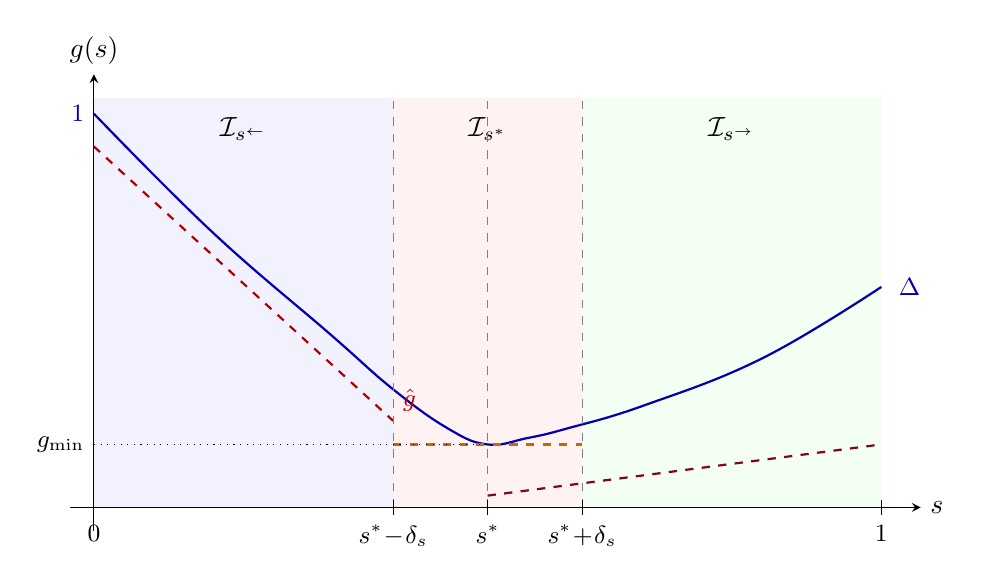
\begin{tikzpicture}[scale=1.0, >=stealth]
  % Axes
  \draw[->] (-0.3,0) -- (10.5,0) node[right] {$s$};
  \draw[->] (0,-0.3) -- (0,5.5) node[above] {$g(s)$};

  % Key positions
  \def\sstar{5.0}
  \def\dsl{1.2}
  \def\dsr{1.2}
  \def\gmin{0.8}
  \def\ghat{1.1}

  % Region shading
  \fill[blue!5] (0,0) rectangle (\sstar-\dsl,5.2);
  \fill[red!5] (\sstar-\dsl,0) rectangle (\sstar+\dsr,5.2);
  \fill[green!5] (\sstar+\dsr,0) rectangle (10,5.2);

  % Region labels
  \node at ({(\sstar-\dsl)/2}, 4.8) {$\mathcal{I}_{s^\leftarrow}$};
  \node at (\sstar, 4.8) {$\mathcal{I}_{s^*}$};
  \node at ({(\sstar+\dsr+10)/2}, 4.8) {$\mathcal{I}_{s^\rightarrow}$};

  % Exact gap (asymmetric: steep left arm, shallow right arm)
  \draw[thick, blue!70!black] plot[smooth, tension=0.7] coordinates {
    (0, 5.0)
    (1.5, 3.5)
    (3.0, 2.2)
    (3.8, 1.5)
    (4.5, 1.0)
    (\sstar, \gmin)
    (5.5, 0.88)
    (6.0, 1.0)
    (7.0, 1.3)
    (8.5, 1.9)
    (10, 2.8)
  };

  % Lower bounds (dashed)
  % Left: g(s) >= A_1(A_1+1)/A_2 * (s*-s), equals g_hat at s*-delta_s
  \draw[dashed, thick, red!70!black] (0, {(\sstar)*\ghat/\dsl}) -- (\sstar-\dsl, \ghat);

  % Window: horizontal at g_min
  \draw[dashed, thick, orange!80!black] (\sstar-\dsl, \gmin) -- (\sstar+\dsr, \gmin);

  % Right: g(s) >= Delta/30 * (s-s_0)/(1-s_0), slope controlled by Delta
  \draw[dashed, thick, purple!70!black] (\sstar, 0.15) -- (10, 0.80);

  % Vertical dashed lines at region boundaries
  \draw[thin, dashed, gray] (\sstar-\dsl, 0) -- (\sstar-\dsl, 5.2);
  \draw[thin, dashed, gray] (\sstar, 0) -- (\sstar, 5.2);
  \draw[thin, dashed, gray] (\sstar+\dsr, 0) -- (\sstar+\dsr, 5.2);

  % Tick marks
  \draw (0, 0.1) -- (0, -0.1) node[below, font=\small] {$0$};
  \draw (\sstar-\dsl, 0.1) -- (\sstar-\dsl, -0.1) node[below, font=\small] {$s^*\!-\!\delta_s$};
  \draw (\sstar, 0.1) -- (\sstar, -0.1) node[below, font=\small] {$s^*$};
  \draw (\sstar+\dsr, 0.1) -- (\sstar+\dsr, -0.1) node[below, font=\small] {$s^*\!+\!\delta_s$};
  \draw (10, 0.1) -- (10, -0.1) node[below, font=\small] {$1$};

  % g_min label
  \draw[thin, dotted] (0, \gmin) -- (\sstar, \gmin);
  \node[left, font=\small] at (0, \gmin) {$g_{\min}$};

  % g_hat label at window boundary
  \node[red!70!black, above right, font=\small] at (\sstar-\dsl, \ghat) {$\hat{g}$};

  % Endpoint values
  \node[blue!70!black, left, font=\small] at (0, 5.0) {$1$};
  \node[blue!70!black, right, font=\small] at (10.1, 2.8) {$\Delta$};
\end{tikzpicture}
\caption{Schematic gap profile for $H(s)$. The solid curve shows the true spectral gap $g(s)$, which equals $1$ at $s=0$, dips to $g_{\min}$ at $s = s^*$, and recovers to $\Delta$ at $s=1$. The left arm is steep (slope $A_1(A_1+1)/A_2$); the right arm is shallower (slope controlled by $\Delta$). Dashed lines show the piecewise lower bounds from \autoref{thm:complete-profile}: linear on the left, constant $g_{\min}$ in the window, and linear on the right (reaching $\Delta/30$ at $s=1$). The right bound is below $g_{\min}$ at $s^*$ but remains $O(g_{\min})$.}
\label{fig:gap-profile}
\end{figure}

Given any problem Hamiltonian $H_z$ satisfying the spectral condition, the gap is bounded across $[0,1]$ by the piecewise profile of \autoref{thm:complete-profile}, determined up to constant factors by $A_1$, $A_2$, $d_0$, and $\Delta$. The minimum gap $g_{\min} = \Theta(\sqrt{d_0/(NA_2)})$ occurs at $s^* = A_1/(A_1+1)$ and is exponentially small in $n$ when $d_0 = O(1)$. The crossing position depends only on $A_1$, not on $A_2$ or $d_0$. More solutions (larger $d_0$) widen the gap; richer spectral structure (larger $A_2$) narrows it. The gap reaches $\Delta$ at $s = 1$, the spectral gap of the problem Hamiltonian itself.

For the running example, the exact gap $g(s) = \sqrt{(2s-1)^2 + 4s(1-s)/N}$ and the piecewise bound from \autoref{thm:complete-profile} can be compared directly. The left bound has slope $(2N-1)/N \approx 2$, matching the asymptotic slope of the exact gap, which approaches $2(1-1/N) \approx 2$ away from $s^*$. The window bound $g_{\min} = 1/\sqrt{N}$ is exact. The right bound has slope approximately $1/15$ near $s^*$, weaker than the true slope by a factor of $30$, but sufficient for the runtime integral since the window dominates.

The runtime integral $\int_0^1 g(s)^{-2}\,ds$ splits across the three regions. In the left and right regions, $g(s) \sim C|s - s^*|$ for constants $C$, and
\begin{equation}
\int_{\delta_s}^{s^*} \frac{du}{(Cu)^2} = \frac{1}{C^2}\left(\frac{1}{\delta_s} - \frac{1}{s^*}\right) \leq \frac{1}{C^2\delta_s},
\end{equation}
which is $O(1/(C^2\delta_s))$. In the window, $g(s) \geq g_{\min}$ gives $\int_{s^*-\delta_s}^{s^*+\delta_s} g(s)^{-2}\,ds \leq 2\delta_s/g_{\min}^2$. The window contribution $\delta_s/g_{\min}^2 = \Theta(A_2^{3/2}/(A_1(A_1+1)) \cdot \sqrt{N/d_0})$ dominates the outer regions, and the full integral --- including the $\Delta$-dependent right-arm contribution --- yields the runtime $T = O((\sqrt{A_2}/(A_1(A_1+1)\Delta^2))\sqrt{N/d_0})$ that Chapter 7 derives rigorously.
